\documentclass[a4paper]{llncs}
\usepackage[utf8]{inputenc}
\usepackage{times,verbatim} % Please do not comment this
\usepackage{graphicx}
\graphicspath{ {images/} }

\begin{document}
	
	\pagestyle{empty}
	
	\mainmatter
	
	\title{Cybersecurity in IT-Scientist Network Infrastructures by
		Honeypots: Catching Cyber Threat Passively}
	% El título no se entiende bien. Voy a por un issue. - JJ
	\titlerunning{Cybersecurity in IT-Scientific Network Infrastructures by Honeypots}
	
	\author{Juan Luis Martin Acal \and Pedro A. Castillo Valdivieso
		\and Gustavo Romero López \and Juan Julián Merelo Guervós \and Pablo García Sánchez }
	
	\authorrunning{Juan Luis Martin Acal}
	
	\institute{Springer-Verlag, Computer Science Editorial III,
		Postfach 10 52 80,\\
		69042 Heidelberg, Germany\\
		\email{jlmacal@correo.ugr.es}\\
		\email{\{pcv, gustavo, jmerelo, pablogarcia\}@ugr.es}\\
		\texttt{http://www.springer.de/comp/lncs/index.html}
	}
	
	\maketitle
	
\begin{abstract}
When dealing with security concerns in the use of IT infrastructures a good balance between security concerns and the right to privacy should be maintained. This is very important in scientific networks, because they were created with an open and decentralized philosophy, in favour of the transmission of knowledge, when security was not a essential topic.
% Deberías hablar de las universidades en el título. NO IT-scientist - JJ
%FERGU: Bueno, y aunque no está mal del todo, en papers en inglés deberías citar papers en inglés. Busca una referencia equivalente a la que usas, pero en inglés, que queda más fino.
Although private and scientific information have a enormous value for an attacker, the user privacy for legal and ethical reasons must be respected. For this reason passive detection methods in cybersecurity such as honeypots are a good strategy to achieve this balance between security and privacy in the defence plan of a scientific network. In this paper we present the practical case of the University of Granada in the application of honeypots for the detection and study of intrusions which avoid intrusive techniques such as the direct analysis of the traffic through networking devices. 
\end{abstract}
	
	
\section{Introduction}
From the earliest days of communication networks, these have been experiencing continuously increasing number of attacks\cite{esset-tendencias,cni-ccn-tendencias-2014,cni-ccn-tendencias-2015}. Also, the complexity of these attacks against the information and resources in the networks has increased. This increase is motivated by  economic, politic or military interests or by the same entities interested in exercise a bigger control over communication freedom in The Internet\cite{cni-ccn-tendencias-2015,cisco-2014}.
	
Although private and scientific information have a enormous value for an attacker, the user privacy for legal and ethical reasons must be respected. Scientific networks are a special and interesting case, in one hand there is a strong demand of security in the network and the resources and services which are listening. On the other hand, the end users demand privacy in his network traffic covered by the law. But it was not designed thinking in security concerns\cite{iris-proyecto}. In contrast to the corporate networks which usually have grown from the intranet to the internet and which have the most of hosts behind the demilitarized zone (DMZ), the scientist networks were born with a open philosophy without focusing on security\cite{iris-proyecto}. Only technical requirements such as the limited number of public IPs forced it to expand private services to the intranet. The information related to research, patents, computer and human resources is a juicy target for hostile agents. Also, the big size of the DMZ makes it prone to a massive attack and increases the possibility of finding a security breach or hide advanced vectors of attack. In this scene the honeypots have an important role in the detection and protection against cyber attacks.

The rest of the paper is organized as follows. In the section \ref{sec:deployment} we expose the characteristic of the passive sensor and the infrastructure used. In the section \ref{sec:analysis}, we present the analysis of the registered data. We make a critical analysis of the strong and weak points for the infrastructure exposed. In section \ref{sec:Strengths&Weaknesse} explains some experiments with machine learning based in S.O.M in order to improve the data analysis. Finally, we present concluding remarks and suggestions for future study.


\section{Deployment of a Security System Based in Honeypots}
\label{sec:deployment}
This section describes the deploy of the system responsible for detecting the malicious activity in the network infrastructure and its components.

\subsection{Honeypots}
A honeypot is a trap that exposes itself. While the honeypot is scanned, probed or compromised by a cyber attack, is collecting information about the malicious activity. There are different classification characteristics such as interaction, distribution appearance or role in multi-tier architecture\cite{Seifert06taxonomyof}. The interaction is the degree of fidelity in the response of the trap. The distribution appearance describes whether the honeypot system appears to be confined to one system or multiple systems. Role, describes in what {\it role} acts within a multi-level architecture and can be server o client.

There is not an ideal configuration of correct features of them, as there exist a huge effect on the nature of the treats and the infrastructure to protect. For example in software development environments, high interaction are used for testing new products with {\it fuzzers} or another type of Penetration Testing (also called {\it pentesting}) tool \cite{fuzzingforsec} in order to discover potential vulnerabilities. On the other hand, low interaction honeypots are used like intrusion detection systems, warning about activity of scans or jumping attempts from compromised internal hosts within production environments. Both share a common point: they are not intrusive with the network traffic.The architecture of the deployed system is divided in two fronts:
\begin{itemize}
	\item The management front has the task to help the operator to manage all the information belong to security incidents and consults it.
	\item The detection front is based on honeypots of medium and low interaction with stand-alone distribution appearance and server role.
\end{itemize}


The sensors were deployed in different production subnets and each one included honeypot software. Specifically Dionaea\cite{dionaea} and Kippo\cite{kippo} which are low and medium interaction honeypot respectively. Each sensor has local data bases with the purpose of saving efficiently the information about attacks, while is waiting to dump the data in the collector. This is  in order to keep the information by duplicate and not to increase the network traffic in case of massive scans or attacks. In the time-lapse for dumped from each sensor to the centralized database, the sensors send incidents by mean of the Linux client of the messaging software ``Telegram'' to the operator, in time-lapses lower than 5 minutes. The collector is a corporate database that feeds the incidents management system and the source of the data analysed.
	
%PONER GRAFICO
	
\section{Data analysis}
\label{sec:analysis}
In this section we expose the analysis of the information gathered and the behavior of detected cyber threats. We explain how this information shows the stages of the complex threats involved in multivector attacks and we discover the finality behind of advanced threats.

For three years each sensor collected information of more of half million of connections. The analysis of this high amount of information has provided the next facts:
\begin{itemize}
	\item External attacks are more frequent than internal attacks.
	\item In one hand the most frequent type of external attacks was weak credentials disclosure. On the other hand the most frequent type of internal attacks was malware propagation.
	\item Countries outside NATO are the most active in the process of scanning and searching for vulnerabilities but curiously most of the intrusions come from NATO member or member candidate countries. It is important to note that this data is dependent on the geolocation of where they are taken.
	\item 
	%la primeroa fase de los ataques son automatizadas.
	%la explotacion es automatizada con supervision humana o humana
\end{itemize}
	
The collected data shows us how external attacks are the most frequent source of attacks. This matches with studies of big security IT enterprises\cite{verizon-2015}. When we studied in detail the information, we saw many connections, some of them from scans to the network infrastructure and others looking for exploiting vulnerabilities or services without strong credentials. About the latter ones is necessary to emphasize those that showed a more advanced level in the process of intrusion because were linked to Advance persistent threats (APT). One of the greatest dangers for IT infrastructures of governments, public administrations and companies are advanced persistence threats. A cyber threat is persistent if it is continuous in time and establishes monitoring and control mechanisms with a hostile agent. It is advanced if uses mechanisms in order to hide its activity in the system. Usually APT are related with cyberspying and elite groups of cybercrime and they are attacks directed against a specific infrastructure. For this reason, it is a priority to detect and study them.

\begin{figure}[h]
	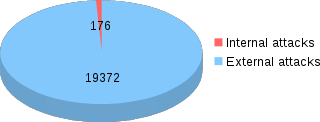
\includegraphics[width=0.5\textwidth]{dionaeaInternalExternal.png}
	\label{fig:intvsextDionaea}
	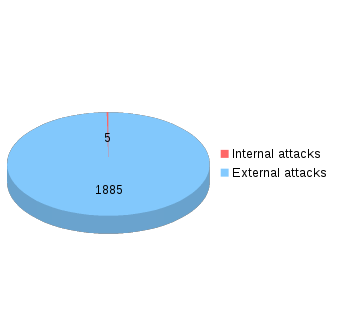
\includegraphics[width=0.5\textwidth]{kippoInternalExternal.png}
	\label{fig:intvsextKippo}
	\caption{On the left, the number of IP involved in external attacks versus internal attacks detected by Dionaea. On the right, the number of IP involved in external attacks versus internal attacks detected by Kippo.}
\end{figure}

The attempts of malware propagation usually belong to advanced and persistent threats and come accompanied by a multivector attack. A attack is multivector whether it exploits multiple vulnerabilities in order to reach its goals. When a Windows host belonging to the infrastructure was compromised by a USB drive, after had communicated its incorporation to the command and control server of the netbot, it started to scan its neighbors within the subnet. Then, it established connections with the sensors that  emulated the ms08-067\cite{ms08067} vulnerability. After this, it commanded to the honeypot software download the binary of trojan from a external web servers. This strategy avoided that firewalls blocked external infections to internal hosts through Server Message Block protocol (SMB) services. Finally, the infected host, not honeypots in our case, would tried to spread the infection, scanning and attacking others subnets, process that is called {\it jumping}.

\begin{figure}[h]
	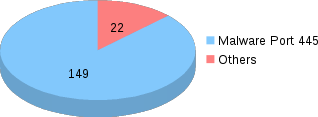
\includegraphics[width=0.5\textwidth]{internalTypes.png}
	\centering
	\label{fig:internalTypes}
	\caption{The malware was main source of internal attacks, and shows a advanced behavior involved in multivector attacks.}
\end{figure}

It is quite difficult follow the clue for rebuilding of multivector attacks. Usually the exploitation of SSH or MySQL weak credentials was the first step to gain the control or access to data in the emulated server. But only a very reduced part shows a clever behavior behind the attack. Between hundred of thousand of connections only a few ones shows access to the fake information such as fake passwords. Then, intelligent attacker tried to use this information against other services with the purpose of  ``jumping'' inside them. A bit more frequent is the attempt to privilege elevation. But the common behavior is to use the basic vulnerability in order to use his network and computational resources as soon as possible. This resources were collected for using in tasks like miner Litecoin\cite{litecoin}, increase the number of nodes for other network scans, for a future deny of service (DoS) attack or for using the compromised host like a anonymous proxy.

When we rebuild the trace of the attack, the first advanced behavior that we find is the use of different hosts for scanning the infrastructure and change to others hosts for the exploitation. The attack starts to scan subnets usually from countries without collaborations accord, in our case China but finally the exploitation is from Europe or United States.%los root kits, los usuarios ocultos,
	
\section{Strengths and Weaknesses of Honeypots}
\label{sec:Strengths&Weaknesse}
The strengths of honeypot are were:
\begin{itemize}
	\item It was not intrusive with network traffic, remained the privacy of infrastructure users. This is a important point because any try of to catch indirect traffic of network would been seen as a threat by other users and a infringement of the use conditions of the network and legality.
	\item The computational and economic resources needed for passive detection are lower because we have only the traffic belong to a potential cyber threat. This an alternative approach to other solutions more expensive like intrusion detection systems based in hardware.
	\item Cyber threats such as advanced malware uses ciphered communications in order to dodge detection systems in the network layer, the only way to catch information its from inside of the compromised node. This is essential if we want analyse how persistence cyber threaths monitor the compromised host and what informations sent outside to its C\&C network.
\end{itemize}
	
The weakness of the honeypot are:
\begin{itemize}
	\item There are many cyber threats focused in the network layer, usually related with deny of services and spoofing. This information is very valuable because this kind of attack are a very important element not only in simple vector attacks, in multivector advanced and persistent attacks too. Honeypots only fetch information from the application layer so they lose essential information for reconstruction of complex attacks.
	\item The use of passive sensors in a security system must be planned with some extra considerations respect the use of active methods of detection. Those considerations cover strategies of deception and hiding of the sensors and politics of migrations in the infrastructure for avoiding it's location.
	\begin{itemize}
		\item Like others deception tools, honeypots must show itself like interesting target for a attacker and avoid them to be easily recognizable by fingerprint techniques. Default installations and configurations in low an medium interaction honeypot are easily detected by a human attacker or a intelligent threat like advanced malware.
		\item When attacker has knowledge of the infrastructure, honeypots are easily dodged so must be deployed together with politics of use like change its subnets or IP every so often.
		\item High interaction honeypots are dangerous in production environments because the monitored sensor is completely real and all his potential in order to attack its periphery. Usually they are deploying in isolated subnets with outgoing traffic strongly restricted in company of others honeypots, that configuration is called honeynet.
	\end{itemize}
\end{itemize}
	
\section{Experiments with S.O.M}
\label{sec:Improve}
In this section, we expose an experiment with Self-Organizing Maps in order to classify information and we comment some interesting results.

In order to classify the information of detected attacks, we apply the classification method that is described in \ cite {}, in two subsets of data. The first advantage is the simplification of the collected information that it derived from the dimensional reduction intrinsic to the method. The attacks are organized in clusters 2D.  This allows identify some very interesting characteristics. The first thing that drawing our attention is how the attacks to HTTP, Microsoft SQL Server (MSSQL) and Session Initiation Protocol (SIP) are concentrated in areas better defined. It is because the cyberthreat showed less variability in their dimensional components. This is explained by the nature of the connections of the attacks and the characteristics of the software used. A sweep scan to search for services in parallel with tools such as Nmap citarXXXXXXXXXXXXXXXx or malware with a very aggressive behavior, have a great variability in the component, source port. On the other hand when the connection comes from targeted attacks or malware behavior shows a discrete to avoid intrusion detection systems, variability is lower.

\section{Conclusion and Future Works}
\label{sec:conclusion&future}
HAY QUE METER MACHINE LEARNING Y MINERIA DE DATOS DE LA BUENA A ESTOS DISPOSITIVOS.

\bibliographystyle{splncs03}
\bibliography{articuloHoneypot}

\end{document}
